\section{ZFS}\label{zfs}

\textbf{fonte}:
\href{https://openzfs.github.io/openzfs-docs/Basic\%20Concepts/Copy-on-write.html}{\url{https://openzfs.org/wiki/System_Administration}}
\url{https://blog.victormendonca.com/2020/11/03/zfs-for-dummies/}

Uno dei principi fondamentali di ZFS:

\begin{quote}
Un blocco in uso non viene mai sovrascritto.
\end{quote}

Modificare dati vuol dire dunque scrivere il nuovo contenuto in una
nuova porzione di memoria, ed il filesystem dovra puntare a questa nuova
area.

Questo principio, permette di implementare e gestire facilmente feature
piu "avanzate" come snapshots ed il self-healing.

\subsection{pool}\label{pool}

Una pool e\textquotesingle{} come un grande albero:

\begin{itemize}
\tightlist
\item
  le foglie contengono i dati
\item
  i nodi interiori sono dei \textbf{block pointers}
\end{itemize}

\textbf{block pointer}: un block pointer tiene traccia di in quali
record si trova il figlio, la grandezza e la \textbf{checksum}.

\begin{itemize}
\tightlist
\item
  \textbf{checksum}: un block pointer contiene la checksum dei nodi
  figli
\end{itemize}

\textbf{uberblock}: e\textquotesingle{} il nodo radice, tutta la pool
e\textquotesingle{} navigabile a partire da qui.

modificare i dati nel filesystem vuol dire ricostruire la catena dei
padri a partire dalla foglia:

\begin{itemize}
\tightlist
\item
  \(D_{4}\) viene liberato, a meno che uno snapshot non lo contenga.{]}
\item
  \(D_{4}'\) e\textquotesingle{} il blocco \(D_{4}\) modificato.
\item
  La modifica a \(D_{4}\) scatena il ricalcolo della checksum e il
  cambio dei puntatori al blocco dati in \(\text{ind 2}\)
\item
  La modifica alla checksum in \(\text{ind2}\) scatena il ricalcolo
  delle checksum di \(\text{root}\)
\item
  ecc.
\end{itemize}

dopo la modifica otteniamo \(\text{uberblock'}\), la nuova radice che
descrive il filesystem con i dati \(D_{4}'\). L\textquotesingle intera
operazione descritta e\textquotesingle{} \textbf{atomica}.

Il costo per una modifica nella pool e\textquotesingle{} proporzionale
alla profondita dell\textquotesingle albero, che non e\textquotesingle{}
necessariamente legato alla grandezza in byte della pool. Il vecchio
albero inoltre risiede ancora in memoria per poterne effettuare uno
snapshot

\subsection{transaction groups}\label{transaction-groups}

Le transazioni sul filesystem sono raggruppate in transaction groups:
\textbf{txg}. L\textquotesingle intero gruppo viene eseguito
atomicamente.

Se un tipo di transazione accumula troppi \emph{dirty data} oppure fa
scattare un timeout (di default di 5 secondi), la transazione viene
annullata ed il file system ritorna all\textquotesingle ultimo albero
per cui e\textquotesingle{} stato fatto il commit.

\begin{quote}
L\textquotesingle ultimo commit potrebbe non essere esattamente
l\textquotesingle albero con i dati piu recenti. Tutta via analizzando
il log prodotto dal file system: ZFS Intent, si possono recuperare le
differenze.
\end{quote}

\subsection{vantaggi di pool e
transazioni}\label{vantaggi-di-pool-e-transazioni}

\textbf{Gli snapshot del filesystem vengono eseguiti a costo quasi
zero}. Fare uno snapshot vuol dire, chiedere al filesystem di non
liberare i dati delle foglie se questi devono essere eliminati o
modificati in versioni future dell\textquotesingle albero.

\textbf{Clonare costa poco in memoria}: basta un riferimento allo stesso
blocco.

ZFS tiene traccia per ogni blocco del \textbf{txg} che lo ha creato,
dunque ZFS puo\textquotesingle{} facilemente identificare quali blocchi
sono stati creati tra uno snapshot e l\textquotesingle altro.

ZFS e\textquotesingle{} in grado di identificare gli erorri nei blocchi
grazie al controllo della corrispettiva checksum che risiede nel padre.
Se nella pool esiste una copia, ridondante dei dati, allora ZFS
puo\textquotesingle{} automaticamente ripristinarne il contenuto.

\subsection{quando ZFS costa in
memoria?}\label{quando-zfs-costa-in-memoria}

\textbf{Frammentazione}: modificare un file vuol dire allocare qua e la
nella pool nuovi blocchi. Dunque modificare un blocco in ZFS vuol dire
rompere la sequenzialità dei blocchi nel file system. Ne consegue che le
performance di ZFS dipendono da quanto spazio libero
c\textquotesingle e\textquotesingle{} nella pool.

\begin{quote}
Se la pool e\textquotesingle{} vuota allora trovare spazio contiguo
e\textquotesingle{} facile, altrimenti l\textquotesingle allocatore deve
lavorare di piu per trovare spazio per nuovi dati.
\end{quote}

Per fare qualsiasi modifica, anche un\textquotesingle eliminazione, ZFS
ha bisogno di memoria.

Per fare una modifica parziale ad un record, bisogna leggerlo,
modificarlo e scriverlo dentro un nuovo record. Dunque piccole modifiche
possono essere molto costose.

\section{struttura di una pool}\label{struttura-di-una-pool}

\subsection{\texorpdfstring{\texttt{vdev}}{vdev}}\label{vdev}

Un vedv (virtual device) e\textquotesingle{} un blocco fondamentale in
ZFS. E\textquotesingle{} un raggruppamento logico di device di dati
fisici (hard disk, ssd, ecc...)

una \textbf{foglia vdev} e\textquotesingle{} il un tipo di vdev che
corrisponde ad uno storage fisico, ossia l\textquotesingle endpoint
nella gerarchia dei tipi di storage in ZFS.

I \passthrough{\lstinline!top-level vdevs!}, sono i device figli del
\passthrough{\lstinline!root vdev!}. Possono essere device singoli,
oppure gruppi logici che raggrupano piu \textbf{foglie}
\passthrough{\lstinline!vdevs!}.

La \passthrough{\lstinline!root vdev!} si trova in cima alla gerarchia
della pool, ed aggrega i vdev figli in un\textquotesingle unica unita di
storage, ossia la pool.


\begin{figure}[htbp]
  \centering
  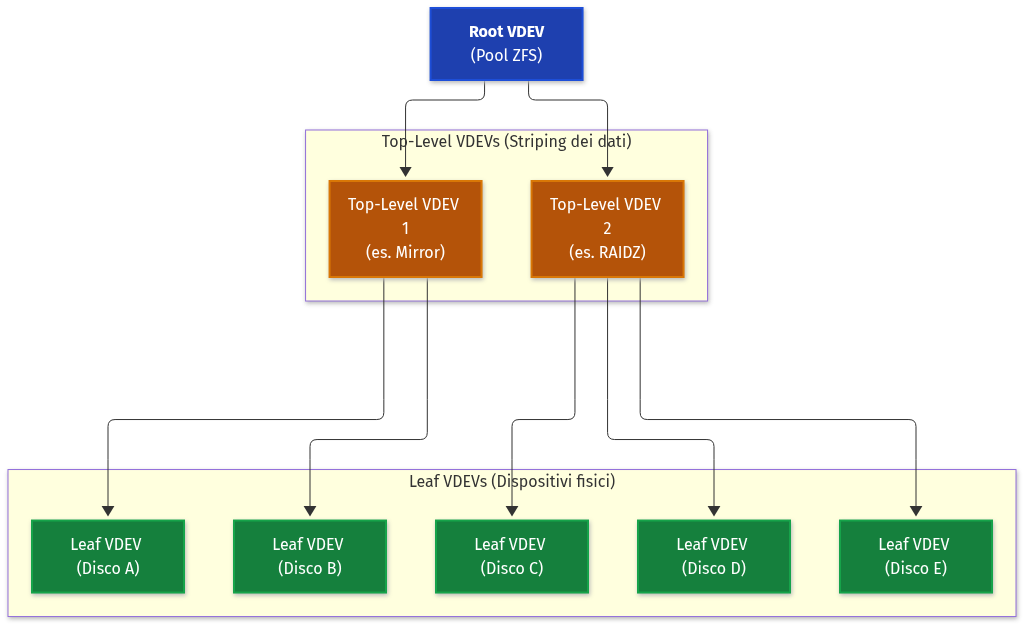
\includegraphics[width=0.92\linewidth,height=0.7\textheight,keepaspectratio]{src/images/mermaid_vdev_bb98e6738a.png}
  \caption{Vdev}
  \label{fig:mermaid_vdev_bb98e6738a}
\end{figure}


Ci sono diversi tipi di \passthrough{\lstinline!vdevs!}:

\begin{itemize}
\tightlist
\item
  \textbf{single device}: rappresenta un singolo disco, file o
  partizione usata a livell di top-level vdev. non dispone di meccanismi
  di ridondanza.
\item
  \textbf{mirror}: e\textquotesingle{} un vdev che tiene in memoria gli
  stessi dati su uno o piu dispositivi per ridondanza.
\item
  \textbf{RAIDZ}: un vdev che offre ridondanza e fault tollerance.
\item
  \textbf{dRAID}: un vdev che offre parita distribuita.
\end{itemize}

Ci sono altri tipi di \passthrough{\lstinline!vdev!}, tra cui:

\begin{itemize}
\tightlist
\item
  \textbf{Spare}: un dispositivo che rimpiazza dispositivi che
  falliscono.
\item
  \textbf{Cache}: un dispositivo utilizzato per fare il cache di dati
  utilizzati frequentemente nalla pool. Mantiene le copie dei dati gia
  presenti nella pool, dunque se un giorno esplode non
  e\textquotesingle{} un problema.
\end{itemize}

\subsection{quindi a che serve un
vdev?}\label{quindi-a-che-serve-un-vdev}

I vdev sono i blocchi fondamentali di una pool ZFS. Il modo in cui i
vdev sono orchestrati determinano le performance del sistema, la
capacita e la ridondanza dei dati.

\section{dataset}\label{dataset}

Una pool e\textquotesingle{} una pila di spazio, i dataset descrivono il
modo in cui lo spazio viene suddivso. Creare un dataset
e\textquotesingle{} un\textquotesingle operazione leggera e non comporta
allocazione.

tipi di dataset:

\begin{itemize}
\tightlist
\item
  \textbf{file system}: un file system POSIX montato-.
\item
  \textbf{volume}: un dispositivo a blocchi usato per macchine virtuali
  swap e file system non supportati da ZFS.
\item
  \textbf{snapshot}.
\end{itemize}

i dataset formano una \textbf{gerarchia}. questa gerarchia rispecchia i
nomi dei dataset e le proprieta vengono ereditate da questa gerarchia.

\begin{lstlisting}[language=bash]
zfs create pool/home
zfs create pool/home/alice
zfs create -V 40G pool/vm/disk0        # a zvol

zfs list                               # file systems and volumes
zfs list -t all -r pool                # everything, recursively
zfs destroy pool/home/alice
\end{lstlisting}

\section{snapshots}\label{snapshots}

creare uno snapshot vuol dire creare un albero che punta ai blocchi di
dati che erano "\textbf{in vita}" al momento dello snapshot.

Uno snapshot e\textquotesingle{} una copia read-only del sistema o di un
volume ad un determinato istante. Creare uno snapshot
e\textquotesingle{} un\textquotesingle operazione quasi istantanea, non
consuma spazio ed e\textquotesingle{} atomica anche se ricorsiva (ossia
sono coinvolti piu dataset)

uno snapshot e\textquotesingle{} raggiungibile tramite la cartella
\passthrough{\lstinline!.zfs/snapshot!}

\begin{quote}
il restore di un file da uno snapshot si fa in questo modo:
\passthrough{\lstinline!cp /home/user/.zfs/snapshot/.../notes.txt /home/user/notes.txt!}
\end{quote}

il comando \passthrough{\lstinline!zfs rollback!} permette di scartare
le modifiche effettuate dall\textquotesingle ultimo snapshot e di
tornare a quel determinato stato.

\subsection{clones}\label{clones}

Un clone e\textquotesingle{} un dataset scrivibile, i cui contenuti
iniziali sono quelli di uno snapshot. Come uno snapshot, il clone
inizialmente non consuma memoria, e poi comincia a divergere rispetto
all\textquotesingle origine con l\textquotesingle aumentare delle
modifiche effettuate.
